\documentclass{article}
\usepackage[rgb]{xcolor}
\usepackage{tikz}
\begin{document}
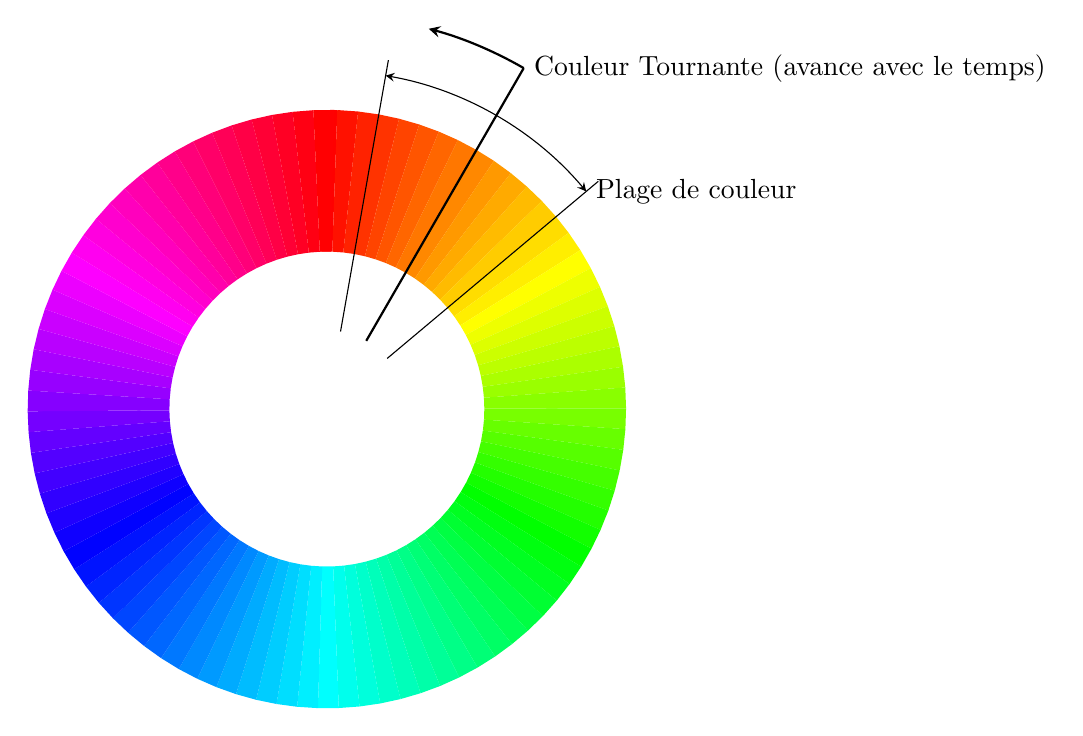
\begin{tikzpicture}[>=stealth]


	% hue circle
	\foreach \x in {0,0.0111,...,1} {
		\definecolor{currentcolor}{hsb}{\x, 1, 1}
		\draw[draw=none, fill=currentcolor]
		(-360*\x+88:2) -- (-360*\x+88:3.8)
		-- (-360*\x+92:3.8) -- (-360*\x+92:2) -- cycle;
	}

	\draw[thick] (60:1) -- (60:5) node[right] {Couleur Tournante (avance avec le temps)};
	\draw[thick, ->] (60:5) arc (60:75:5);



	\draw (40:1) -- (40:4.5);
	\draw (80:1) -- (80:4.5);

	\draw[<->] (0,0) ++(80:4.3) arc (80:40:4.3) node[right] {Plage de couleur};



\end{tikzpicture}

\end{document}
